%versi 2 (8-10-2016)
\chapter{Landasan Teori}
\label{chap:teori}

\section{IDE UNPAR}
\label{sec:IDE UNPAR} 

IDE UNPAR (\textit{Interactive Digital learning Enviroment}) dibangun dengan tujuan untuk menjawab tantangan dan peluang dari fenomena \textit{Massive Open Online Courses}\cite{IDE:dasar-dasar}. IDE UNPAR memiliki fitur-fitur untuk membantu pembelajaran berbasi \textit{e-learning} yang akan dibahas di dalam subbab-subbab berikut ini.

\subsection{Mengelola Mata Kuliah}
Mata kuliah adalah komponen yang penting ketika akan menjalankan pembelajaran secara daring. IDE UNPAR memiliki fitur untuk membantu pengajar menyusun mata kuliah yang akan diajar.  Fitur mengelola mata kuliah IDE UNPAR memungkinkan pengajar untuk menambahkan kerangka kuliah, silabus, dan lain-lain.

Fitur mengelola mata kuliah juga memungkinkan dosen untuk menambahkan buku untuk sebagai sumber pembelajaran, menggungah file agar mahasiswa peserta mata kuliah tersebut dapat mengakses dokumen-dokumen yang digunakan dan dibagikan oleh dosen, menambahkan folder untuk menyusun file-file yang akan digunakan dalam proyek mahasiswa atau tempat berbagi file antara dosen pengajar dalam satu mata kuliah, penambahan tautan untuk menyediakan sumber untuk mahasiswa dalam bentuk halaman web, menambahkan label untuk memberi informasi tambahan pada suatu aktivitas di dalam mata kuliah, membuat \textit{page} untuk menyatukan informasi-informasi terkait suatu topic mata kuliah di dalam satu tempat.

\subsection{Mengelola Kelas} 
Fitur mnegelola kelas memungkinkan dosen untuk mengelompokkan mahasiswa peserta mata kuliah dengan tujuan memberikan tugas kepada masing- masing kelompok, atau ketika suatu mata kuliah diampu oleh dua dosen atau lebih sehingga ada pembagian mahasiswa yang akan diajar oleh kedua dosen tersebut.

\textit{Group} pada IDE terbagi menjadi dua, yaitu \textit{seperate} dan \textit{visible}. Perbedaan dari kedua jenis \textit{group} tersebeut adalah, \textit{seperate group} menghalangi anggota satu grup melihat diskusi grup lainnya, sedangkan \textit{visible groups} memungkinkan anggota suatu grup untuk melihat diskusi dari grup lainnya. Indikator \textit{group} dapat dilihat ketika membuat sebuah aktivitas. Ikon akan muncul seperti gambar \ref{fig:groups}.

\begin{figure} 
	\centering  
	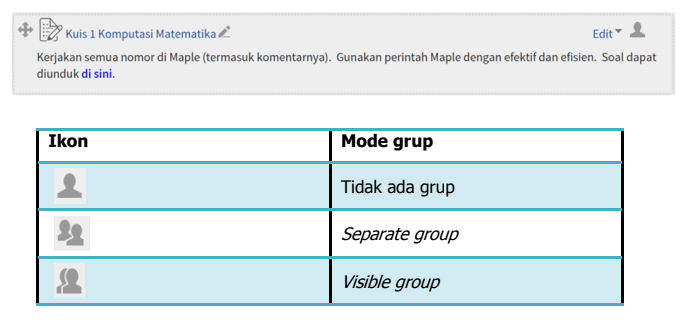
\includegraphics[scale=0.5]{activity-group.png}  
	\caption[Gambar aktivitas dalam IDE] {Gambar aktivitas dalam IDE\cite{IDE:dasar-dasar}} 
	\label{fig:groups} 
\end{figure} 
Fitur mengelola kelas juga meiliki fungsi laporan atau \textit{reports}. IDE UNPAR akan menyediakan laporan aktivitas apa saja yang dilakukan oleh mahasiswa dan dapat dilihat oleh dosen pengampu mata kuliah tersebut. Laporan yang disediakan oleh IDE UNPAR dapat membantu dosen untuk menentukan \textit{recourse} atau aktivitas mana saja yang lebih menarik untuk mahasiswa penempuh mata kuliah.

\subsection{Forum dan Pesan}
Fitur forum menyediakan tempat untuk mahasiswa dan dosen melakukan sesi diskusi yang dapat dilihat oleh semua yang mengikuti mata kuliah tersebut. Forum juga memungkinkan dosen untuk memberikan pengumuman terkait matakuliah yang diampu agar dapat dilihat oleh semua mahasiswa peserta mata kuliah. Fitur forum dari IDE UNPAR juga bersifat asinkronus sehingga peserta dalam forum tidak diharuskan \textit{online} diwaktu yang bersamaan.

Fitur pesan atau \textit{messages} dari IDE UNPAR berbeda dengan fitru forum karena fitur pesan bersifat sinkronus, sehingga pihak yang terkait harus \textit{online} secara bersamaan. Fitur pesan hanya dapat dilihat oleh dua pihak yang sedang terkait. Fitur pesan dapat digunakan untuk bertukar informasi antara dosen dan mahasiswa, atau sesama mahasiswa. Membuat pesan dapat dilakukan dengan memilih \textit{messages} pada blok \textit{messages}, kemudian akan muncul halam seperti pada gambar \ref{fig:messages}. Pencarian kontak dapat dilakukan dengan memilih menu \textit{dropdown} yang bertuliskan \textit{Contacts} atau dengan menggunakan \textit{search bar}.
\begin{figure} [H]
	\centering  
	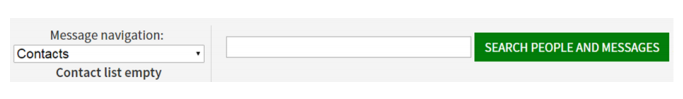
\includegraphics[scale=0.5]{messages-page}  
	\caption[Halaman \textit{messages} dalam IDE] {Halaman \textit{messages} dalam IDE\cite{IDE:dasar-dasar}}
	\label{fig:messages} 
\end{figure} 
   

\subsection{Tugas dan Kuis}
Tugas dan kuis juga menjadi salah satu komponen yang penting dari suatu mata kuliah. Fitur tugas memungkinkan mahasiswa untuk mengumpulkan submisi dari tugas yang telah diberikan oleh dosen pengampu mata kuliah. Dosen pengampu mata kuliah tersebut juga dapat menentukan batas pengumpulan tugas yang diberikan, menilai dan memberi komentar kepada submisi tugas mahasiswa dan mengunduh seluruh submsisi mahasiswa pada mata kuliah tersebut dengan mudah.

Fitur kuis pada IDE UNPAR dapat merancang kuis dalam bentuk pilihan ganda, jawaban singkat, benar atau salah, dan lain-lain\cite{IDE:dasar-dasar}. Fitur kuis juga memungkinkan dosen untuk mengatur lamanya pengerjaan kuis, pembatasan akses kuis, pembatasan kelompok yang dapat menempu kuis, dan pembatasan jumlah pengerjaan kuis.  Dosen juga dapat memilih untuk memberikan \textit{feedback} atau menunjukkan jawaban yang benar kepada peserta kuis.

Nilai dari suatu tugas dalam IDE dapat dimasukkan dengan dua cara. Cara pertama dapat dilakukan dengan menekan pilhan yang dilingkarkan nomor 2 pada gambar \ref{fig:grading}. Cara kedua dapat dilakukan dengan menekan pilihan yang dilingkarkan nomor 3 pada gambar \ref{fig:grading}, cara ini akan mengunduh semua tugas mahasiswa. Rangkuman niliai tugas mahasiswa dapat dilihat oleh dosen dengan memilih menu yang dilingkari nomor 1 pada gambar \ref{fig:grading}.
\begin{figure} [ht]
	\centering  
	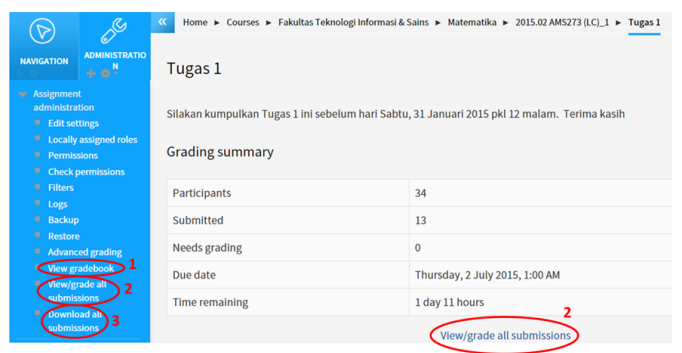
\includegraphics[scale=0.5]{assignment-grading.png}  
	\caption[Halaman nilai tugas dalam IDE] {Halaman nilai tugas dalam IDE\cite{IDE:dasar-dasar}} 
	\label{fig:grading} 
\end{figure}
\section{Moodle}
\label{sec:Moodle}

Moodle (\textit{Modular Object-Oriented Dynamic Learning Environment}\cite{moodle:39}) pertama di kembangkan oleh Martin Dougiamas dan dirilis pada 20 Agustus 2002\cite{moodle:39}. Tujuan dari Moodle adalah untuk augmentasi dan memindahkan pembelajaran bersifat \textit{offline} menjadi {online}. Moodle dibangun dengan panduan pandangan \textit{social constructist pedagogy}\cite{moodle:39}. Pandangan Moodle membantu mereka untuk membuat \textit{ Learning Management System} yang memiliki fokus pembelajaran dari sudut pandang pelajar. Tidak hanya digunakan dalam lingkungan pendidikan, Moodle juga digunakan di dalam lingkungan seperti pelatihan, pengembangan, dan bisnis.

Struktur moodle disusun di sekitar \textit{course}. Struktur Moodle biasanya berupa sebuah halaman atau area di dalam platform moodle dimana pengajar dapat memberika aktivitas atau sumber pembeljaran kepada peserta dari \textit{course} mereka.\textit{Course} yang dimaksud adalah mata pelajara, mata kuliah, atau topik pelajaran apapun yang digunakan oleh yayasan yang menggunakan Moodle. 

Moodle bersifat modular sehingga Moodle dibentuk sebagai sebuah aplikasi pusat, dimana bisa ditambahkan plugin untuk memasukkan sebuah fitur baru yang spesifik seperti plugin autentikasi dan plugin aktivitas di dalam \textit{course}. Setiap jenis plugin yang berbeda akan berkomunikasi dengan inti Moodle melalui API yang berbeda. Moodle tidak hanya menyediakan fitur-fitur spesifik yang berbeda, Moodle juga menyediakan pengubahan tema tampilan. Pengubahan tema pada Moodle bekerja tidak jauh dengan cara bekerja plugin. Tema di dalam Moodle juga berada pada level yang berbeda yaitu tema Moodle secara keseluruhan, tema spesifik dari \textit{course}, dan tema dari semua \textit{course} dari suatu kategori. \cite{moodle:dev}

Moodle telah mencapai dan mematuhi standar internasional sebagai berikut : \cite{moodle:39}
		\begin{enumerate}
			\item \textbf{\textit{An Open Source Initiative}} \\
				Moodle disediakan sebagai perangkat lunak \textit{open source} yang dapat digunakan dan dimodifikasi secara gratis dibawah lisensi \textit{\textit{GNU General Public License}}.
			\item \textbf{IMS LTI\texttrademark} \\
				Moodle telah memenuhi standar untuk integrasi aplikasi pembelajaran, sehingga pengguna dapar mengitegrasikan dan menyajikan aplikasi dan konten yang dihosting secara eksternal.
			\item \textbf{\textit{SCORM-ADL}} \\
				Moodle memungkinkan penggunanya untuk mengirimkan konten SCORM (\textit{Shareable Content Object Reference Model}) dengan mengunggah paket SCORM atau AICC ke dalam \textit{course} Moodle.
	
			\item \textbf{\textit{Open Badges}} \\
				Open Badges milik Mozilla mendukung dan menstandarisasi pemblajaran secara daring dengan menggunakan \textit{badges}. Moodle telah mengitegrasikan fitur tersebut sehingga institusi, organisasi, atau individu dapat membuat dan membagikan \textit{badges} kepada pelajar di platform Moodle.
		\end{enumerate}

Lisensi Moodle, yaitu \textit{GNU GENERAL PUBLIC LICENSE Version 3, 29 June 2007} menyatakan secara eksplisit pada bagian pembukaan bahwa lisensi tersebut menjamin kebebasan untuk membagi dan mengubah semua versi dari aplikasi agar aplikasi tersebut bersifat gratis untuk seluruh penggunanya\cite{GNU:preamble}.

\section{Moodle mobile}
\label{sec:Moodle mobile}
Moodle mobile dikembangkan menggunakan Ionic, karena Ionic memungkinkan pengembangan aplikasi yang bersifat \textit{cross-platform}\cite{Ionic:intro}. Sifat \textit{cross-platform} dari Ionic membuat Moodle mobile dengan mudah diterapkan ke berbagai platform dengan hanya satu \textit{codebase}. Pengembangan aplikasi dengan \textit{view} yang besar akan lebih cepat dengan penggembangan \textit{framework} bersifat \textit{cross-platform} dibandingkan dengan pengembangan secara \textit{native} \cite{cross-platform}. 

Ionic memungkinkan Moodle mobile untuk bekerja seperti aplikasi \textit{native} karena Ionic menggunakan Cordova. Cordova adalah sebuah \textit{framework} pengembangan aplikasi mobile yang bersifat \textit{open source}. Cordova memungkinkan pengembangan aplikasi mobile dengan menggunakan teknologi standar web. Aplikasi yang dikembangkan dengan menggunakan Cordova akan bergantung kepada binding API yang sesuai standar untuk mengakses kemampuan setiap perangkat seperti sensor, data, status jaringan dan lain-lain\cite{cordova:overview}. Ionic juga dapat dikembangkan dengan integrasi bersama \textit{framework} lain seperti Angular atau React. Moodle mobile versi 3.5 dikembangkan menggunakan Ionic versi 3 \cite{moodle:dev}. Ionic versi 3 masih menggunakan Angular secara langsung, sehingga Moodle mobile dikembangkan dengan Ionic yang diintegrasikan dengan Angular \cite{moodle:dev}.


Moodle mobile bersifat modular seperti Moodle berbasis web yang berarti Moodle mobile juga mendukung \textit{themes} dan \textit{plugins}. \textit{Plugin} akan membantu pengembang menambahkan fitur dengan mudah ke dalam aplikasi Moodle mobile. \textit{Themes} memungkinkan pengembang Moodle mobile untuk mengubah gaya dan layout dari aplikasi Moodle mobile sesuai dengan keinginannya. Pada subbab-subbab berikut akan dibahas mengenai fitur-fitur, \textit{plugin}, dan \textit{theme} dari Moodle mobile.
\subsection{\textit{Themes} dan \textit{Plugins}}
\textit{Themes} dan \textit{plugins} pada Moodle mobile bekerja berbeda dengan Moodle berbasis web. Perbedaan yang ada dari Moodle berbasis web dengan Moodle mobile diantaranya adalah \textit{themes} dan \textit{plugin}.Pada Moodle mobile sebelum versi 3.5 \textit{themes} yang sudah digunakan pada Moodle web akan secara otomatis digunakan juga pada Moodle mobile. Moodle mobile versi 3.5 dan seterusnya sudah tidak dapat mendukung penggunaan \textit{themes} lagi karena Ionic versi 3 tidak mendukung \textit{custom themes} dari Moodle sebelum versi 3.5.\cite{moodle:dev}. Sehingga untuk mengubah tampilan dari Moodle mobile adalah dengan mengubah source code Moodle mobile sendiri. Awalnya \textit{plugin} pada Moodle mobile sebelum versi 3.5 dapat bekerja dengan membuat modul Angular atau Ionic lalu menambahkannya pada bagian \textit{plugin} di dalam Moodle mobile. Semenjak Moodle mobile versi 3.5 plugin dapat digunakan tanpa harus membuat modul Angular atau Ionic, pengembang aplikasi cukup membuat template plugin menggunakan PHP dan \textit{markup} Ionic 3\cite{moodle:dev}. \textit{Plugin} pada Moodle mobile juga dapat dibagi menjadi tiga jenis dengan cara bekerja yang berbeda-beda. Tiga jenis \textit{plugin} pada Moodle mobile yaitu :

	\begin{enumerate}
	\item Template \textit{plugin} yang dihasilkan dan diunduh ketika pengguna membuka \textit{plugin}-nya\\
		Template \textit{plugin} ini akan mulai diproses ketika pengguna akan membuka \textit{plugin}-nya. Fungsi yang dipanggil dari template ini akan menerima beberapa parameter \textit{context}.
		
	\item Template \textit{plugin} yang diunduh ketika pengguna \textit{login} dan di-\textit{render} menggunakan data dari JavaScript \\
		Template \textit{plugin} ini  akan mulai diproses ketika pengguna \textit{login} ke dalam Moodle mobile dan template akan disimpan ke dalam perangkat pengguna. Fungsi dari template \textit{plugin} ini tidak akan menerima parameter \textit{context} seperti pada template \textit{plugin} sebelumnya.
	\item \textit{Plugin} yang dibuat hanya menggunaka JavaScript \\
		\textit{Plugin} ini akan bekerja sesuai dengan bagaiamana pengembang aplikasi membuatnya, karena \textit{plugin} ini tidak menggunakan API dari Moodle.
	\end{enumerate}

\subsection{Fitur-fitur}
Moodle mobile menyediakan fitur-fitur yang serupa dengan Moodle berbasis web untuk membantu melakukan pembelajaran secara daring. Fitur-fitur yang disediakan oleh Moodle mobile beberapa ada yang dapat bekerja secar luring. Berikut adalah beberapa fitur yang disediakan oleh Moodle mobile \cite{moodle:39}:

	\begin{enumerate}
		\item \textit{See your courses at a glance} \\
			Fitur ini akan menampilkan semua \textit{courses} yang sedang di tempuh dalam bentuk \textit{ion-card} di halam utama Moodle mobile. \textit{Courses} yand ditampilkan juga akan dipisah %more explanation here
			dan pengguna juga dapat memfilter \textit{courses} yang ditempuh. Fitur ini juga dapat digunakan di dalam kondisi luring.
		\item \textit{Easily access course content} \\
			Pengguna dapat mengakses konten dari seluruh \textit{courses} yang ditempuh melalui \textit{courses} yang ditampilkan pada halaman utama. Fitur ini dapat digunakan dalam kondisi luring.
		\item \textit{View and access activities which are due} \\
			Fitur ini dapat diakses melalui tab \textit{timeline}. Tab \textit{timeline} akan menunjukkan aktivitas-aktivitas dari \textit{course} yang ditempuh oleh pengguna secara berurut mulai dari tenggat waktu terdekat. Pengguna akan dapat secara langsung mengakses aktivitas-aktivitas yang ditampilkan melalui tab \textit{timeline}. Fitur ini dapat digunakan di dalam kondisi luring.
		\item \textit{Grades and grading} \\
			Moodle mobile akan menyediakan tautan untuk mengakses buku nilai, dan pengajar dapat melihat nilai dari submisi tugas pelajar. Fitur ini dapat digunakan secara luring.
		\item \textit{Grade assignment} \\
			Pengajar dapat memberikan tugas yang mereka berikan melalui Moodle mobile. Fitur ini dapat digunakan secara luring.
		\item \textit{Notes} \\
			Pengajar dapat melihat catatan situs, \textit{courses}, dan catatan pribadi tentang murid mereka. Fitur ini dapat digunakan secara luring.
		\item \textit{Message participants} \\
			Pengguna dapat mengirim pesan pribadi kepada rekan mereka yang menggunakan Moodle atau terdaftar dalam satu \textit{course} yang sama. Fitur ini hanya dapat digunakan secara daring.
		\item \textit{Take quizess on your mobile device} \\
			Pelajar dapat mengerjakan ujian melalui Moodle mobile. Tidak semua ujian dapat dikerjakan melalui Moodle mobile seperti ujian yang membutuhkan \textit{safe browser}, ujian yang memiliki jenis pertanyaan dimana pertanyaa itu hanya dapat dijawab apabila pertanyaan sebelumnya sudah dijawab. Ujian yang menggunakan \textit{plugin} dapat dikerjakan pada Moodle mobile apabila \textit{plugin} tersebut mendukung Moodle mobile.\cite{moodle:39}
			
			Ujian tidak seluruhnya dapat dikerjakan secara luring. Syarat ujian yang dapat dikerjakan diluar luring adalah ujian tanpa batas waktu, pertanyaan ujian berupa umpan balik yang ditangguhkan, tidak ada kebutuhan alamat jaringa. \cite{moodle:39}
	\end{enumerate}
	
Tertulis di atas adalah sebagian dari fitur yang disediakan oleh Moodle mobile beserta ketersediaannya dalam kondisi daring atau luring. Fitur -fitur yang lengkap dapat dilihat pada lampiran yang disediakan.

\section{Moodle mobile Development}
\label{sec:MoodleAppDev}

Selama masa pengembangan Moodle mobile dikategorikan menjadi dua, yaitu Moodle mobile 1 dan Moodle mobile 2 \cite{moodle:dev}. Perbedaan dari kedua versi Moodle mobile ini adalah kelengkapan fitur-fitur yang digunakan dan teknologi yang digunakan. Pada dasarnya kedua versi dari Moodle mobile ini dapat dianggap sebagai \textit{webservice client} yang menggunakan protokol REST untuk mendapatkan dan mengirim informasi dari Moodle ke Moodle mobile. 

\subsection{Moodle mobile 1}
 Moodle mobile 1 pertama kali dirilis pada tanggal 15 april 2013 untuk iOS dan 8 april 2013 untuk Android dengan versi 1.2.1. Versi 1.2.1 digunakan karena fitur-fitur tersedia diwariskan dari aplikasi My Moodle, My Moodle adalah aplikasi khusu iOS yang sudah usang.\cite{moodle:dev}

Moodle mobile 1 dikembangkan tanpa menggunakan Ionic, melainkan dikembangkan dengan teknologi sebagai berikut : \cite{moodle:dev}
	\begin{itemize}
		\item HTML5
		\item CSS3
		\item \textit{Media queries for screen width and height}
		\item Phonegap
		\item jQuery
		\item jQuery UI
		\item jQuery touch swipe
		\item matchMedia
		\item Backbone dan Underscore
		\item RequireJS
		\item jsdoc
		\item Google Javascript Style Guide
		\item Google Closure Lint
	\end{itemize}
Dengan menggunakan teknologi diatas Moodle mobile 1 dapat menggunakan atau mengakses fitur dari perangkat seluler seperti kamera, perekema audio dan vidio, file sistem, dan lain-lain.

Moodle mobile 1 dikembangkan dari versi 1.2.1 sampai dengan versi 1.15 sebelum akhirnya digantikan oleh Moodle mobile 2. Fitur-fitur yang dirilis pada versi-versi Moodle mobile 1 kemudian akan digunakan atau diimplementasi ulang pada Moodle mobile 2. Bagian berikut akan membahas rilis \textit{major} selama Moodle mobile 1 dikembangkan.

\subsubsection{Versi 1.2.1 }
Rilis pertama Moodle mobile 1 dengan fitur-fitur sebagai berikut  :\cite{moodle:dev}
	\begin{itemize}
		\item Desain responsif untuk ponsel dan tablet
		\item Mengunggah file ke dalam area file pribadi
		\item Merekam audio dan mengunggah ke dalam area file pribadi
		\item Mengirim pesan pribadi kepada peserta \textit{courses}
		\item Menulis catatan pribadi
		\item Menelpon peserta \textit{course} lainnya
		\item Mencari alamat peserta \textit{course} lainnya dengan google maps
		\item Mengunduh dan melihat beberapa sumber 
		\item Akses cepat menuju konten \textit{course}
		\item Translasi jarak jauh
		\item Kustomisasi layout dan gaya jarak jauh
	\end{itemize}

Sebagai rilis pertama dari Moodle mobile 1, versi ini didesain dengan kekuatan seperti aplikasi yang aman, dapat bekerja secara luring, dapat mendukung notifikasi, dapat diubah merek dan ekspansi oleh institusi, dan membuat beberapa operasi Moodle lebih cepat dan mudah. \cite{moodle:dev}

\subsubsection{Versi 1.3}
Versi 1.3 dirilis pada 24 september 2013 untuk Android dan iOS, dengan menambahkan fitur-fitur sebagai berikut : \cite{moodle:dev}
	\begin{itemize}
		\item Opsi untuk \textit{refresh} pada menu utama
		\item Sebagian dukungan untuk menjalankan aplikasi pada desktop
		\item Dukungan untuk label teks lengkap
		\item Perbaikan desain secara general
		\item Ikon loading yang kontekstual
		\item Informasi tolongan pada halama login
		\item Menggantikan library jQuery UI dengan dialog HTML5 rancangan sendiri 
	\end{itemize}

\subsubsection{Versi 1.4}
Versi 1.4 dirilis pada 3 maret 2014 untuk Android dan iOS dengan fitur-fitur : \cite{moodle:dev}
	\begin{itemize}
		\item Notifikasi untuk iOS dan Moodle versi 2.7 atau 2.6
		\item Kalender acara
		\item Peringatan saat mengunduh file yang terlalu besar
	\end{itemize}

\subsubsection{Versi 1.5}
Versi 1.5 dirilis pada 18 juli 2014 untuk Android dan iOS dengan tambahan fitur-fitur : \cite{moodle:dev}

	\begin{itemize}
		\item Melihat nilai aktivitas dan hasilnya
		\item Halaman baru untuk sign in dan mengelola akun
	\end{itemize}

Selain fitur-fitur di atas ada beberapa perbaikan juga yand diimplementasi oleh Moodle sebagai berikut :
	\begin{itemize}
		\item URL situs dapat mendukung domain tanpa protokol HTTP atau HTTPS
		\item Perbaikan halaman notifikasi
		\item Pesan yang diterima dapat dibalas secara \textit{in-line}
		\item \textit{Refresh} dapat memperbarui semua informasi terkait situs
		\item Tautan bantuan sekarang merujuk ke dokumentasi sesuai versi yang digunakan
		\item Perbaikan dukungan untuk tema
	\end{itemize}
	
\subsubsection{Versi 1.6}
Versi 1.6 dirilis pada 7 agustus 2014 untuk Android dan iOS dengan fitur-fitur baru sebagai berikut : \cite{moodle:dev}
	\begin{itemize}
		\item Melihat total nilai untuk setiap \textit{course}
		\item Fitur \textit{My files} untuk melihat dan mengunduh file pribadi dan file \textit{courses}
		\item Menu \textit{course} yang dapat dilipat
	\end{itemize}

\subsubsection{Versi 1.7}
Versi 1.7 dirilis pada 10 oktober 2014 dengan fitur-fitur baru sebagai berikut :  \cite{moodle:dev}
	\begin{itemize}
		\item Dukungan untuk aktivitas forum
		\item Seluruh file dalam direktori, halaman atau sumber file dapat diunduh dengan sekali sentuh
		\item Memperbarui bahasa translasi
		\item Memperbarui performa animasi 
	\end{itemize}
\subsubsection{Versi 1.8}
Versi 1.8 dirilis pada 10 november 2014 dengan fitur-fitur baru seperti :\cite{moodle:dev}
	\begin{itemize}
		\item Dukungan untuk Moodle 2.8
		\item Pesan dan notfikasi ditampilkan secara terpisah
		\item HTML dan sumber daya halaman ditampilkan menggunakan \textit{viewer} di dalam aplikasi
		\item Apabila pengguna menekan notifikas, aplikasi akan dibuka dan menunjukkan notfikasi secara lengkap
		\item Judulu notifikasi ditampilkan pada bilah notifikasi Android
	\end{itemize}
\subsubsection{Versi 1.9}
Versi 1.9 dirilis pada 29 november 2014 dengan fitur-fitur baru seperti : \cite{moodle:dev}
	\begin{itemize}
		\item Penambahan bahasa baru
		\item Notifikasi forum lebih ringkas dan mengandung tautan untuk membuka diskus secara langsung
		\item Penambahan tombo \textit{show grades} dalam profil peserta untuk melihat nilai peserta
	\end{itemize}
\subsubsection{Versi 1.10}
Versi 1.10 dirilis pada 26 desember 2014 dengan fitur baru untuk \textit{messages} yaitu antarmuka baru yang serupa dengan WhatsApp atau Telegram, pengguna dapat melihat pesan baru,  mencari kontak, menambah atau menhapus kontak, dan melihat profil pengguna. \cite{moodle:dev}

\subsubsection{Versi 1.11}
Versi 1.11 dirilis pada 16 Januari 2015, dengan fitur-fitur sebagai berikut : \cite{moodle:dev}
	\begin{itemize}
		\item Integrasi kalender dengan pengingat peringatan sebagai notifikas lokal
		\item Bagian ringkasan ditampilkan di dalam halaman konten \textit{courses}
	\end{itemize}

\subsubsection{Versi 1.12}
Versi 1.12 dirilis pada 20 Februari 2015 dengan fitur-fitur sebagai berikut : \cite{moodle:dev}
	\begin{itemize}
		\item Semua tipe file dapat diunggah ke Moodle
		\item Acara grup sekarang ditampilkan pada daftar acara
		\item Opsi pengingat baru untu notifikasi lokal
		\item Menghapus \textit{permissions} yang tidak digunakan dalam Android
		\item Pengguna yang diblokir akan ditampilkan dalam kontak	
		\item Penggun dapat memblokir dan buka blokir dalam opsi \textit{messages}
	\end{itemize}

\subsubsection{Versi 1.13}
Versi 1.13 dirilis pada 27 Maret 2015 dengan fitur-fitur sebagai berikut : \cite{moodle:dev}
	\begin{itemize}
		\item Pengajar dapat melihat submisi tugas murid secara daring dan luring
		\item File dalam iOS dibuka menggunakan \textit{framework} Quick Look
	\end{itemize}

\subsubsection{Versi 1.14}
Versi 1.14 dirilis pada 30 April 2015 dengan fitur-fitur baru dan perbaikan sebagai berikut : \cite{moodle:dev}
	\begin{itemize}
		\item Aktivitas murid ditampilkan pada catatan situs Moodle
		\item Konten dalam aplikasi diproses melalui filter Moodle
		\item Applikasi diperbarui untuk menggunakan fitur dan perbaikan baru dalam Moodle 2.9 
	\end{itemize}

\subsubsection{Versi 1.5}
Versi 1.15 dirilis pada 29 Mei 2015. Versi ini adalah versi terakhir yang dirilis untuk Moodle mobile 1. Berikut adalah fitur-fitur dan perbaikan pada versi 1.15 : \cite{moodle:dev}
	\begin{itemize}
		\item Menghalangi pengguna untuk login ketika fitur mengunduh file tidak diaktifkan di dalam \textit{Mobile service}
		\item Konten sudah ditampilkan dengan benar pada Android 4.4.2
		\item \textit{Plugin} fitur tambahan diperbarui untuk mendukung Moodle 2.9
		\item Mencegah untuk memproses kode js filter Moodle saat merender panel
	\end{itemize}

\subsection{Moodle mobile 2}
Moodle mobile 2 adalah seri lanjutan dari Moodle mobile 1 dengan perubahan utama pada teknologi yang digunakan. Moodle mobile 2 dikembangkan menggunakan \textit{framework} Ionic 1. Moodle mobile 2 juga menggunakan Cordova untuk kompilasi atau pengemasan interaksi dengan perangkat pengguna. Struktur dari Moodle mobile 2 dibagi menjadi dua, yaitu \textit{core} dan \textit{addons}. 

\textit{Core} dan \textit{addons} memiliki struktur yang sama, yaitu struktur standar Angular. \textit{Core} dan \textit{addons} akan memiliki komponen Angular yang diorganisir menjadi \textit{NgModules}\cite{angular:architecture}
. \textit{NgModules} dapat dianggap sebagai wadah untuk untuk kode yang didedikasikan untuk domain aplikasi, \textit{workflow}, atau kapabilitas aplikasi yang bersifat erat. \textit{NgModules} akan menyediakan sebuah kompilasi kontex untuk komponen. \cite{angular:architecture:modules}

Komponen pada Angular akan mengendalikan sepetak \textit{view}, \textit{view} yang dimaksud adalah template pasangan dari komponen Angular tersebut dalam bentuk HTML. Template dari komponen Angular akan memiliki \textit{template syntax} Angular yang dapat digunakan untuk mengubah HTML sesuai dengan logika aplikasi dan keadaan aplikasi dan data DOM. Template tersebut dapat menggunakan \textit{data binding} untuk mengkordinasi apliksai dan data DOM, \textit{pipe} untuk mengubah data sebelum ditampilkan, atau \textit{directives} untuk menerapkan logika aplikasi kepada apa saja yang akan ditampilkan. \cite{angular:architecture:components}

\textit{Core} dan \textit{addons} menjadi wadah untuk fitur yang akan digunakan pada Moodle mobile 2, dengan perbedaan \textit{core} akan menyimpan fitur yang dibutuhkan oleh Moodle mobile 2 atau fitur-fitur dasar dengan struktur Angular yang standar. \textit{Addons} akan berisi fitur yang bukan menjadi fitur utama dari Moodle mobile 2. \cite{moodle:dev}

Moodle mobile 2 menyediakan \textit{directives} bawaan yang dapat digunakan untuk \textit{addons} dan komponen. berikut adalah directives yang disediakan oleh Moodle mobile 2 : \cite{moodle:dev}
\begin{itemize}
\item mmAutoFocus digunakan untuk secara otomatis fokus kepada \textit{input element}.
\item mmBroswser membuat tautan yang ditekan agar terbuka dalam \textit{browser} yang terpisah.
\item mmCompletion akan menyediakan \textit{checkbox} yang menunjukkan status aktivitas.
\item mmExternalContent akan menambahkan seluruh konten eksternal ke dalam antrian untuk diunduh.
\item mmFile digunakan untuk menunjukkan daftar file yang dapat dibukan.
\item mmFormatText akan memproses tulisan yang akan ditampilkan.
\item mmIframe berguna untuk membantu membuka tautan di dalam \textit{iframe} yang bersifat \textit{relative} dan \textit{non-relative}.
\item mmImageViewer berguna untuk membuat sebuah gambar menjadi responsive.
\item mmLoading akan menggantikan konten dengan halaman \textit{loading} dari Moodle ketika Moodle mobile 2 sedang mengambil konten.
\item mmNavigationBar akan menunjuukan bilah navigasi.
\item mmNoInputValidation menonaktifkan validasi otomatis dari bidang \textit{input}.
\item mmSplitView dan mmSplitViewLink memungkinkan Moodle mobile untuk menjalankan fiture \textit{split screen} pada ponsel atau tablet.
\end{itemize}

Moodle mobile 2 mengalami perubahan \textit{framework} menjadi Ionic 3 pada versi 3.5 \cite{moodle:dev}. Perubahan \textit{framework} ini membuat Moodle mobile 2 hanya berjalan pada perangkat bergerak dengan versi Android 4.4 atau iOS 8 dan seterusnya. Perangkat dengan versi sistem operasi sebelum yang disebutkan hanya dapat menjalankan Moodle mobile 2 dengan \textit{framework} Ionic 1. Versi Moodle mobile 2 dibawah versi 3.5 tersebut kemudian dikategorikan oleh Moodle sebagai Moodle Classic App.



\section{Lingkungan Pengembangan Berdasarkan Dokumentasi Moodle}
\label{moodle docs:env}
Kustomisasi Moodle mobile dimulai dengan menyiapkan lingkungan pengembangan agar pengembang dapat mengubah \textit{source code}, melakukan pengujian menggunakan \textit{browser} pada mesin, dan \textit{deploy} aplikasi ke pergangkat seluler. Kebutuhan yang diperlukan untuk menyiapkan lingkungan pengembangan Moodle mobile adalah sebagai berikut : \cite{moodle:dev}


\begin{enumerate}
	\item Adanya \textit{browser} untuk pengembangan.
	\item Git untuk \textit{source control} aplikasi dan \textit{clone} Moodle mobile.
	\item Node.js untuk menjalankan \textit{script} JavaScript tanpa \textit{browser}.
	\item Mesin yang menggunakan sistem operasi Windows akan membutuhkan alat \textit{native build}.
	\item Cocoapods pada Mac untuk mengelola \textit{dependency}.
	\item libsecret untuk sistem operasi linux agar dapat melakukan \textit{push} URL \textit{diff} atau perbedaan antar file dalam \textit{repository} lokal dan \textit{remote}.
	
\end{enumerate}

Langkah pertama menyiapkan kebutuhan lingkungan pengembangan adalah dengan menginstall Node.js. Node yang disarankan oleh dokumentasi Moodle mobile adalah Node.js dengan versi 11\cite{moodle:dev}. Langkah kedua adalah dengan menginstall kebutuhan spesifik yang dibutuhkan oleh Moodle mobile sesuai dengan sistem operasi yang digunakan. Kebutuhan yang dimaksud adalah \textit{Windows native build tools} untuk Windows, \textit{cocoapods} untuk Mac, dan \textit{libsecret} untuk Linux. Langkah ketiga yang harus dilakukan adalah dengan melakukan \textit{clone} dari \textit{branch} Moodle mobile milik Moodle dengan command  \texttt{git clone \url{https://github.com/moodlehq/moodleapp.git}}. Dokumentasi Moodle app menyarankan untuk menggunakan \textit{branch} dengan nama \textit{integration}\cite{moodle:dev}. \textit{Branch integration} digunakan karena dalam \textit{branch} tersebut pengembangan dan \textit{branch} dimana perbaikan-perbaikan terabaru diimplementasikan. Sehingga setelah melakukan \textit{clone} lakukan \textit{checkout} ke \textit{branch Integration}.


Menyiapkan lingkungan pengembangan untuk Moodle app dimulai dengan menginstall Gulp untuk automasi pengembangan tugas, menginstall Ionic, kemudian menjalankan \texttt{npm run setup}, \textit{command} tersebut menjalankan \texttt{npm install}, \texttt{npx cordova prepare}, dan \texttt{npx gulp} yang masing-masing akan menginstall \textit{dependency} npm, menyiapkan cordova, dan menjalankan tugas dasar gulp. Setelah itu jalankan \texttt{npm start} pada folder utama Moodle mobile untuk menjalankan Moodle mobile dalam \textit{browser}.

Uji coba Moodle mobile dengan menggunakan perangkat seluler dapat dilakukan dengan \textit{command} \texttt{npm run dev:android} untuk Android dan \texttt{npm run dev:ios} untuk iOS. Kedua \textit{command} tersebut dijalankan dengan menggunakan Cordova, yang memiliki kebutuhan masing-masing untuk setiap platform. Cordova untuk Android akan membutuhkan Java Development Kit, Gradle, dan Android SDK\cite{cordova:android}. Cordova untuk iOS akan membutuhkan Xcode dan ios-deploy \cite{cordova:iOS}.

Membangun versi produksi aplikasi akan membutuhkan kompilasi dengan AOT (\textit{ahead-of-time}) dari Angular. Untuk melakukan kompilasi AOT ada bebrapa file yang harus dimodifikasi. Perubahan pada file-file berikut diperlukan karena kompilasi standar AOT angular menyebabkan masalah dengan aktivitas \textit{database} dan dukungan Moodle untuk \textit{plugins}.  File yang pertama adalah \texttt{node\_modules/@angular/platform-browser-dynamic/esm5/platform-browser-dynamic.js }, dalam file tersebut variable \texttt{\_NO\_RESOURCE\_LOADER} yang memiliki fungsi \texttt{get} dengan baris seperti pada \mbox{Kode \ref{lst:noresourceloader}} yang akan diubah menjadi seperti pada \mbox{Kode \ref{lst:noresourceloaderreplace}}.\cite{moodle:dev}

\begin{lstlisting}[ frame=single, label={lst:noresourceloader}, language=PHP, caption=Fungsi \texttt{get} pada \textunderscore NO\textunderscore RESOURCE\textunderscore LOADER]
throw new Error
("No ResourceLoader implementation has been provided. 
Can't read the url \"" + url + "\"");
\end{lstlisting}

\begin{lstlisting}[frame=single, label={lst:noresourceloaderreplace}, language=java, caption=Kode pengganti untuk fungsi \texttt{get}]
url = 'templates/' + url;

        var resolve;
        var reject;
        var promise = new Promise(function (res, rej) {
            resolve = res;
            reject = rej;
        });
   var xhr = new XMLHttpRequest();
   xhr.open('GET', url, true);
   xhr.responseType = 'text';
   xhr.onload = function () {
   // responseText is the old-school way of retrieving response 
   //(supported by IE8 & 9)
   // response/responseType properties were introduced in 
   //ResourceLoader Level2 spec (supported by IE10)
   var response = xhr.response || xhr.responseText;
   // normalize IE9 bug (http://bugs.jquery.com/ticket/1450)
  var status = xhr.status === 1223 ? 204 : xhr.status;
  // fix status code when it is 0 (0 status is undocumented).
  // Occurs when accessing file resources or on Android 4.1 stock browser
  // while retrieving files from application cache.
  if (status === 0) {
  status = response ? 200 : 0;
   }
   if (200 <= status && status <= 300) {
       resolve(response);
   }
   else {
       reject("Failed to load " + url);
   }
   };
   xhr.onerror = function () { reject("Failed to load " + url); };
   xhr.send();
   return promise;
\end{lstlisting}

File kedua yang harus dimodifikasi adalah \texttt{node\_modules/@ionic/app-scripts/dist/util/config.js}, pada bagian \texttt{optimizejs} modifikasi sehingga terlihat seperti pada \mbox{Kode \ref{optimizejs}} dengan menghapus \texttt{context.isProd}.
\\
\\

\begin{lstlisting}[frame=single, label={optimizejs}, language=PHP, caption= \texttt{optimizejs} setelah modifikasi]
context.optimizeJs = [
        context.optimizeJs,
        hasArg('--optimizeJs')
    ].find(function (val) { return typeof val === 'boolean'; });
\end{lstlisting}
Setelah modifikasi kedua file tersebut berhasil jalankan \textit{command} \texttt{npm run ionic:build -- --prod} untuk kompilasi. Untuk menginstall pada platform jalankan \textit{command} \texttt{npx cordova run android} untuk Android dan \texttt{npx cordova build ios} untuk iOS.


\section{\textit{Plugin} cordova-pdf-generator}
\label{pdf-gen}
\textit{Plugin} cordova-pdf-generator adalah plugin yang berfungsi untuk menghasilkan sebuah file PDF secara offline. \textit{Plugin} ini mengubah HTML menjadi PDF, dan juga menyediakan mekanisme untuk membagikan PDF ke dalam aplikasi lain seperti Mial dan lain-
lain.\cite{cordova-pdf-generator}

Salah satu fitur dari \textit{plugin} ini adalah mengembalikan file dalam representasi Base64 yang dapat digunakan untuk mengunggah file ke dalam server. Fitur tersebut hanya ada untuk platform Android dan iOS saja. \textit{Plugin} ini juga dapat digunakan bersamaan dengan Ionic dan Angular, sehingga \textit{plguin} ini dapat digunakan untuk mengembangkan fitur \textit{PDF Scanner} pada IDE UNPAR mobile. Contoh penggunaan \textit{plugin} dalam ionic dapat dilihat pada\mbox{Kode \ref{example:pdf-gen}}.

\begin{lstlisting}[language= Java, frame=single, label={example:pdf-gen}, caption= Penggunaan \textit{plugin} pada Ionic dan Angular]
import { Component } from '@angular/core';
 
import { NavController } from 'ionic-angular';
 
declare var cordova:any;    //global;
 
@Component({
  selector: 'page-home',
  templateUrl: 'home.html'
})
export class HomePage {
 
  constructor(public navCtrl: NavController) {
      const before = Date.now();
 
            document.addEventListener('deviceready', () => {
                console.log('DEVICE READY FIRED AFTER', 
		(Date.now() - before), 'ms');
 
                //generate the pdf.
                cordova.plugins.pdf.fromData
	     ( '<html> <h1>  Hello World  </h1> </html>', options )
                .then(()=>'ok')
                .catch((err)=>console.err(err))
  }
 
}
 
\end{lstlisting}

